\section{Architettura del prodotto}

\subsection{Descrizione generale}
Il progetto \textit{Predire in Grafana} prevede la realizzazione di due moduli: un plug-in per la piattaforma Grafana e un tool esterno di supporto, rispettivamente chiamati \textbf{Prediction Plug-in} e \textbf{Training Tool}. \\
Il Training Tool si occupa di addestrare un algoritmo di \textit{SVM} o \textit{Regressione Lineare} utilizzando un dataset inserito dall'utente, per poi generare un file json contenente le informazioni necessarie per poter effettuare un calcolo di predizione. Questo modulo è stato sviluppato seguendo il pattern \textit{Model-View-ViewModel (MVVM)}.\\
Il Prediction Plug-in invece si occuperà di ricevere in input il json e una volta collegati i predittori contenuti nel file ad un flusso dati, permetterà di iniziare ad effettuare i calcoli di previsione. Questo modulo è stato sviluppato seguendo il pattern \textit{Model-View-Controller (MVC)}.\\
Le motivazioni principali che hanno portato alla scelta del design pattern MVVM per il Training Tool sono:
\begin{itemize}
	\item per la realizzazione del componente è stato utilizzato \textit{React} e abbiamo ritenuto che questo pattern si accoppiasse bene con la struttura di \textit{React}.
\end{itemize}
Le motivazioni principali che hanno portato alla scelta del design pattern MVC per il Prediction Plug-in sono:
\begin{itemize}
	\item abbiamo ritenuto che questo pattern si accoppiasse meglio con la struttura dei plug-in di Grafana.
\end{itemize}
Inoltre entrambi i pattern permettono:
\begin{itemize}
	\item di disaccoppiare la parte di \textit{presentation logic} da quella di
\textit{business logic};
	\item il riutilizzo di alcune componenti in altri contesti.
\end{itemize}


\subsubsection{Diagrammi delle attività}
\begin{figure}[H]
\centering
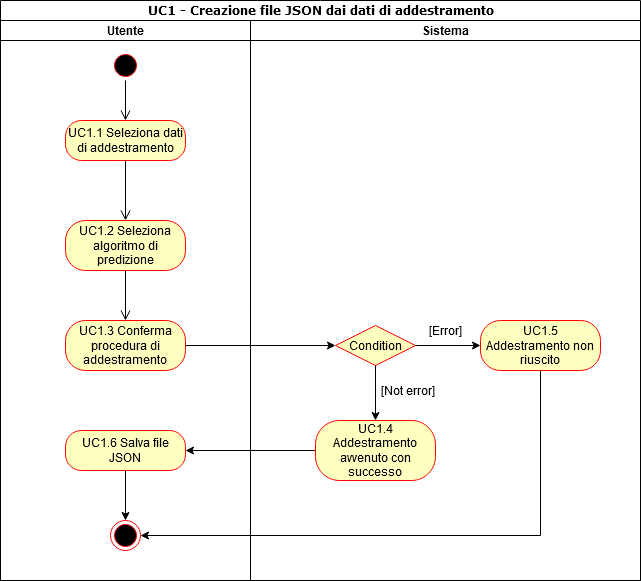
\includegraphics[scale=0.6]{../../Diagrams/Activity_diagrams/uc1.png}
\caption{Diagramma delle attività dello UC1}
\end{figure}
\begin{figure}[H]
\centering
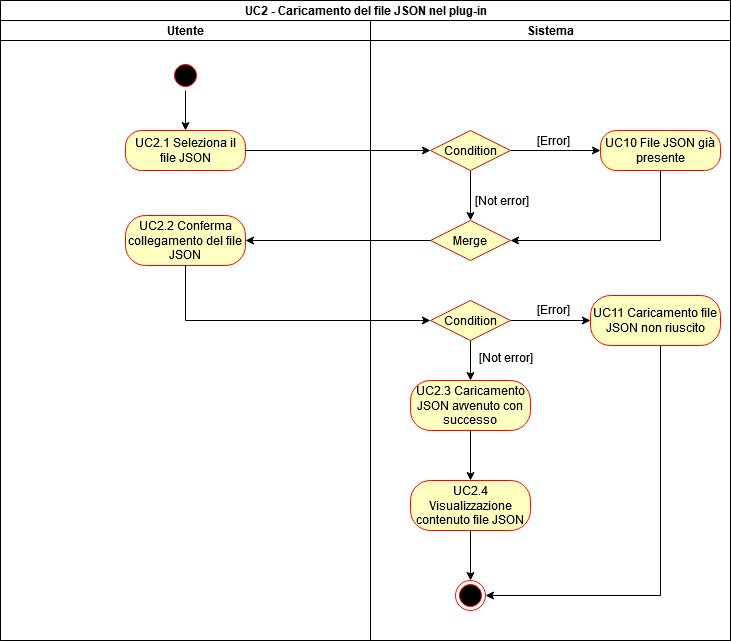
\includegraphics[scale=0.6]{../../Diagrams/Activity_diagrams/uc2.png}
\caption{Diagramma delle attività dello UC2}
\end{figure}
\begin{figure}[H]
\centering
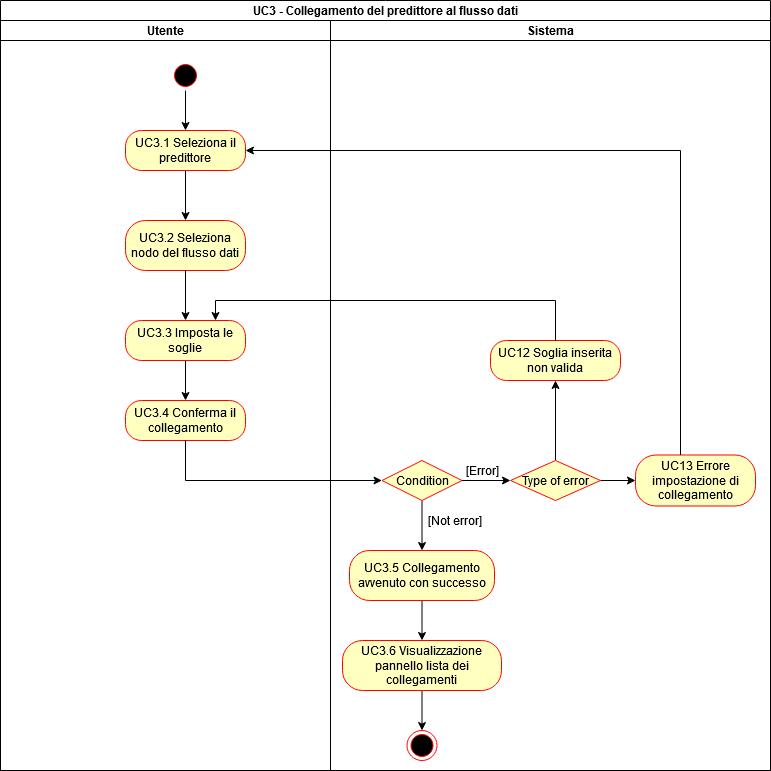
\includegraphics[scale=0.6]{../../Diagrams/Activity_diagrams/uc3.png}
\caption{Diagramma delle attività dello UC3}
\end{figure}
\begin{figure}[H]
\centering
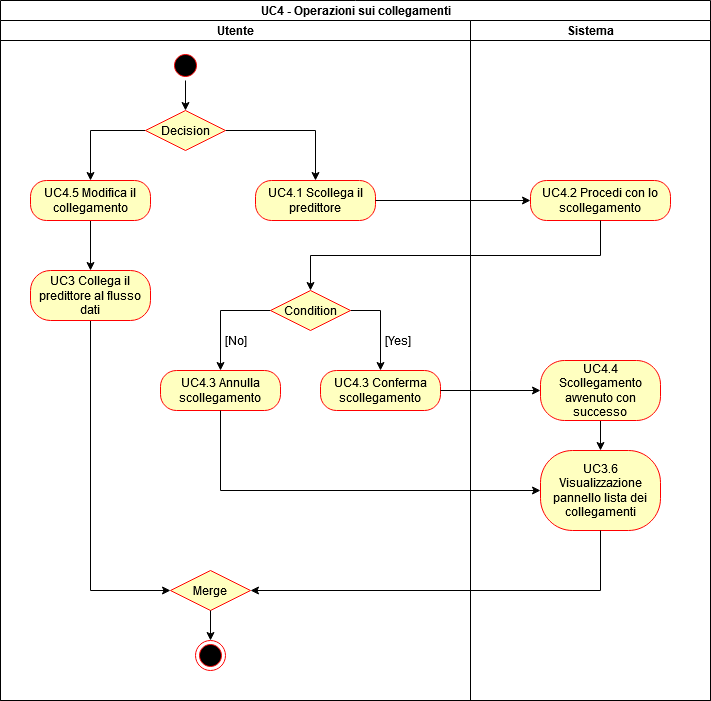
\includegraphics[scale=0.6]{../../Diagrams/Activity_diagrams/uc4.png}
\caption{Diagramma delle attività dello UC4}
\end{figure}
\begin{figure}[H]
\centering
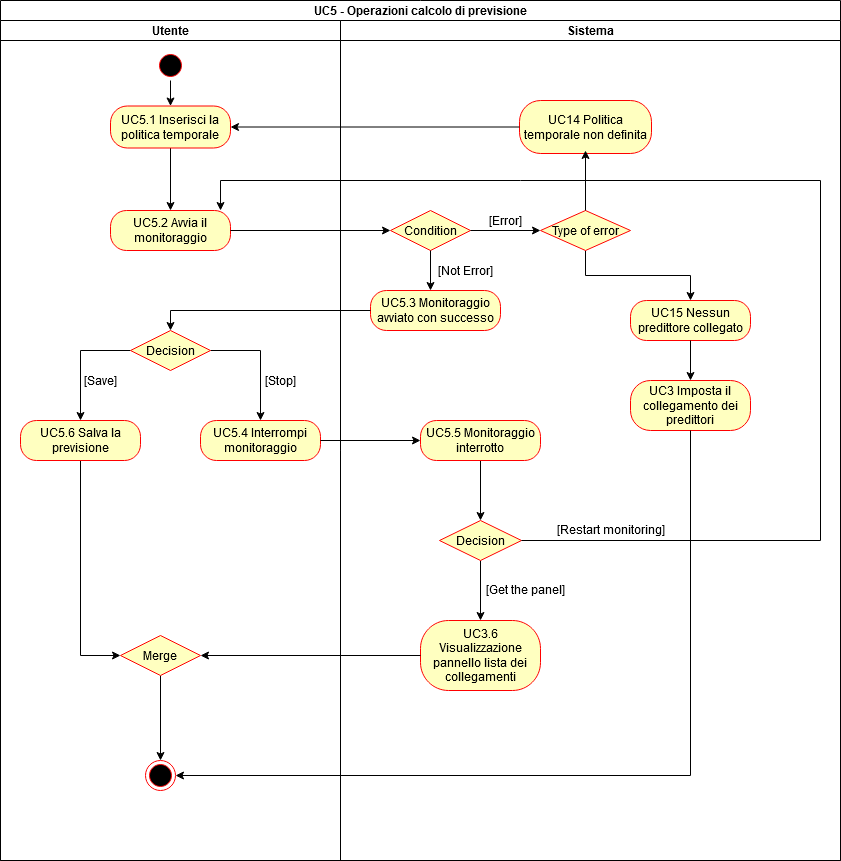
\includegraphics[scale=0.5]{../../Diagrams/Activity_diagrams/uc5.png}
\caption{Diagramma delle attività dello UC5}
\end{figure}
\begin{figure}[H]
\centering
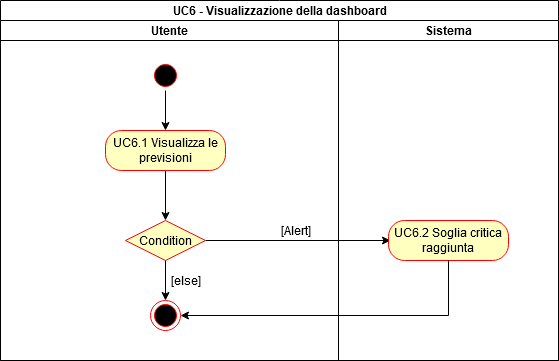
\includegraphics[scale=0.6]{../../Diagrams/Activity_diagrams/uc6.png}
\caption{Diagramma delle attività dello UC6}
\end{figure}

\subsection{Architettura Training Tool}

\subsubsection{Descrizione}
L'implemetenazione del tool è stata realizzata utilizzando il design pattern MVVM.
Il passaggio di dati dalle view al model avviene attraverso la modifica di un campo dati \textit{props} immesso dal \textit{ViewModel}.
Attraverso queste \textit{props} il \textit{ViewModel} chiama le funzioni corrette quando l’utente interagisce con la vista.
La divisione tra Business Logic\glo e Presentation Logic è rafforzato da questo utilizzo delle \texttt{props}.
Nel modello viene fornita funzionalità per la gestione degli algoritmi tramite le classi \textit{SVMtrain} e \textit{RLtrain} che verranno utilizzate dal \textit{ViewModel}.


\begin{comment} si trovano un'istanza delle classi SVMtrain e RLtrain in base all'algoritmo scelto, le classi stesse si trovano nel modello e si occupano di rendere polimorfe le funzioni principali, come quelle di addestramento o di recupero del file JSON.
\end{comment}

\subsubsection{Diagrammi dei package}
\begin{figure}[H]
\centering
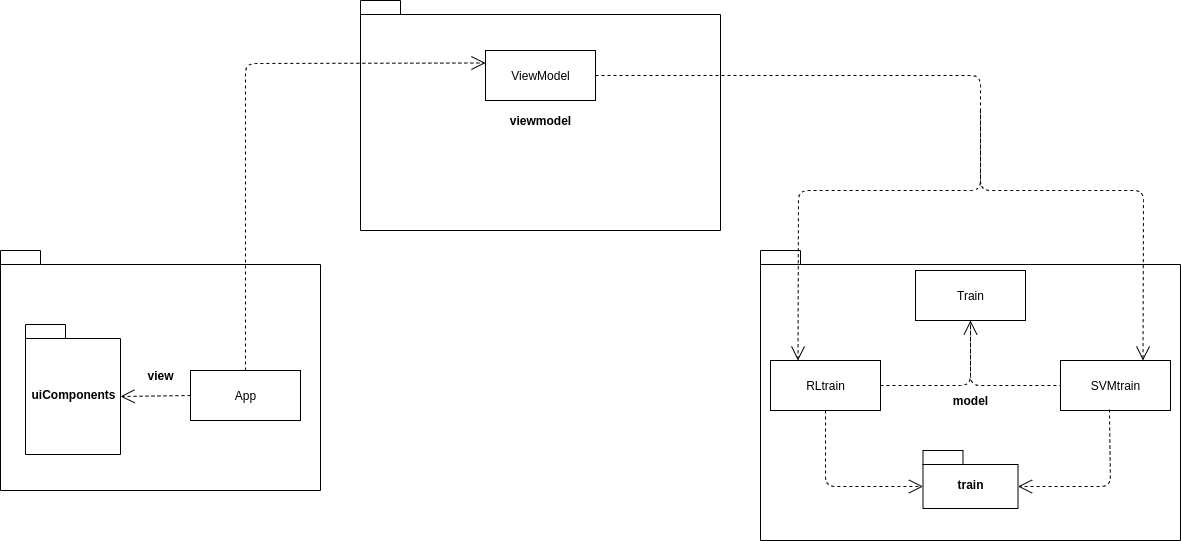
\includegraphics[scale=0.45]{../../Diagrams/Package_diagrams/tool_design_patern.png}
\caption{Diagramma dei package del Training Tool}
\end{figure}

\subsubsection{Diagrammi delle classi}
\textbf{Model}
\begin{figure}[H]
\centering
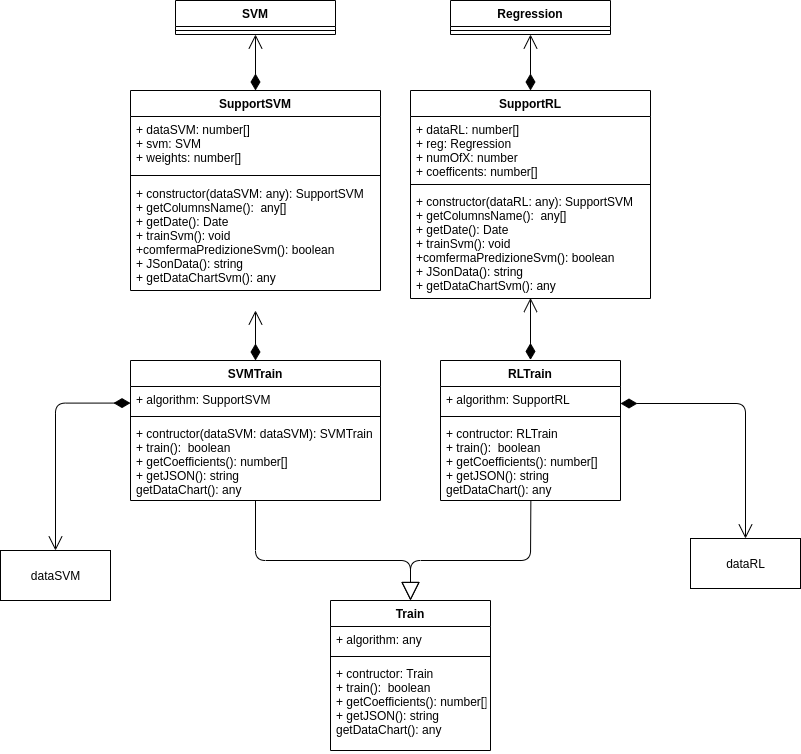
\includegraphics[scale=0.5]{../../Diagrams/Classes_diagrams/tool_model.png}
\caption{Diagramma delle classi del Model del Training Tool}
\end{figure}

\textbf{View}
\begin{figure}[H]
\centering
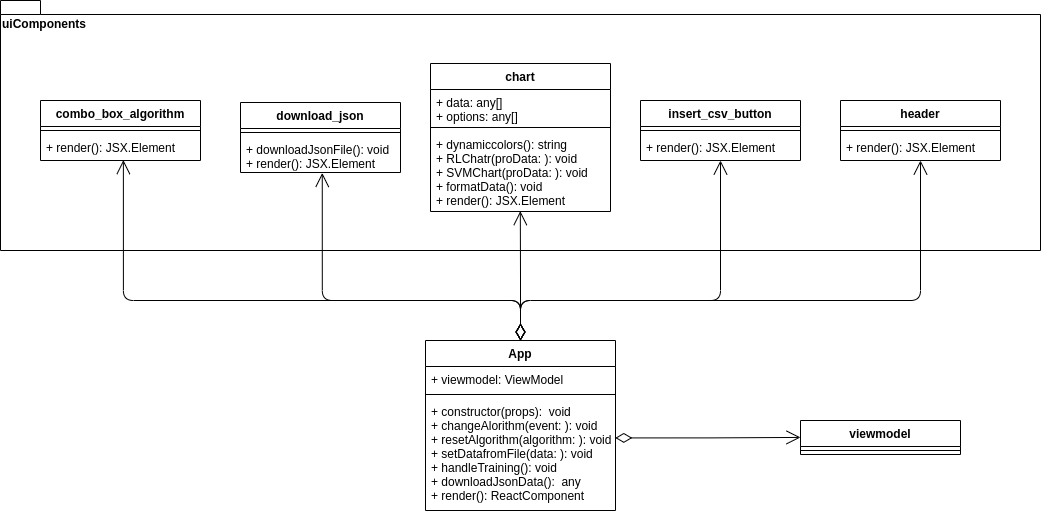
\includegraphics[scale=0.5]{../../Diagrams/Classes_diagrams/tool_view.png}
\caption{Diagramma delle classi della View del Training Tool}
\end{figure}

\textbf{ViewModel}
\begin{figure}[H]
\centering
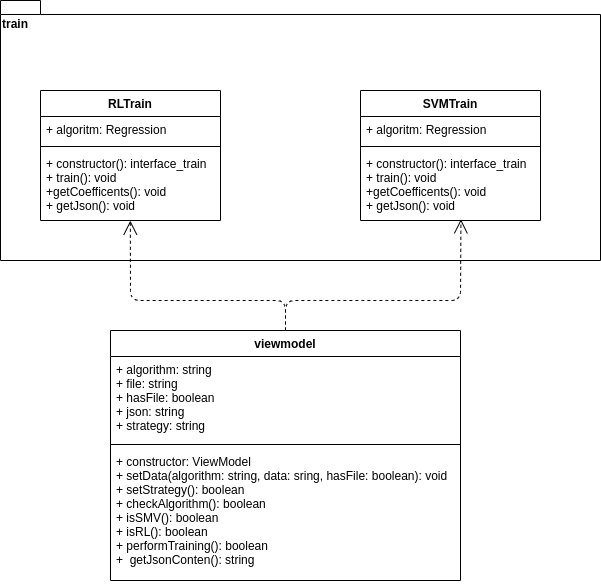
\includegraphics[scale=0.5]{../../Diagrams/Classes_diagrams/tool_modelview.png}
\caption{Diagramma delle classi del ViewModel del Training Tool}
\end{figure}


\subsubsection{Diagrammi di sequenza}
\begin{figure}[H]
\centering
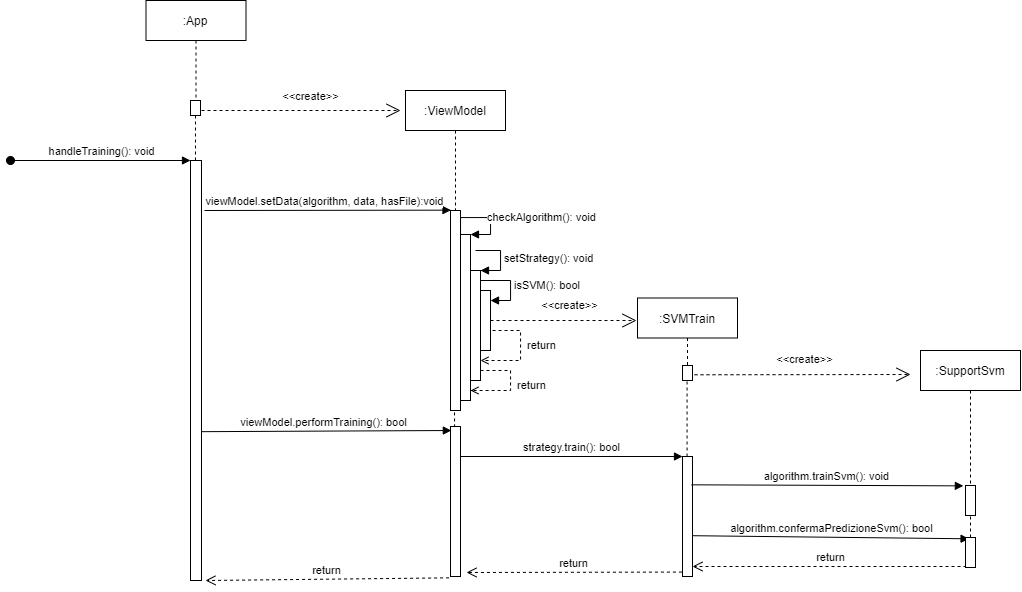
\includegraphics[scale=0.45]{../../Diagrams/Sequence_diagrams/trainSVM.png}
\caption{Diagramma di sequenza del TrainSVM}
\end{figure}

\subsubsection{Design pattern notevoli utilizzati}


\subsection{Architettura Prediction Plug-in}

\subsubsection{Descrizione}

\subsubsection{Diagrammi dei package}
\begin{figure}[H]
\centering
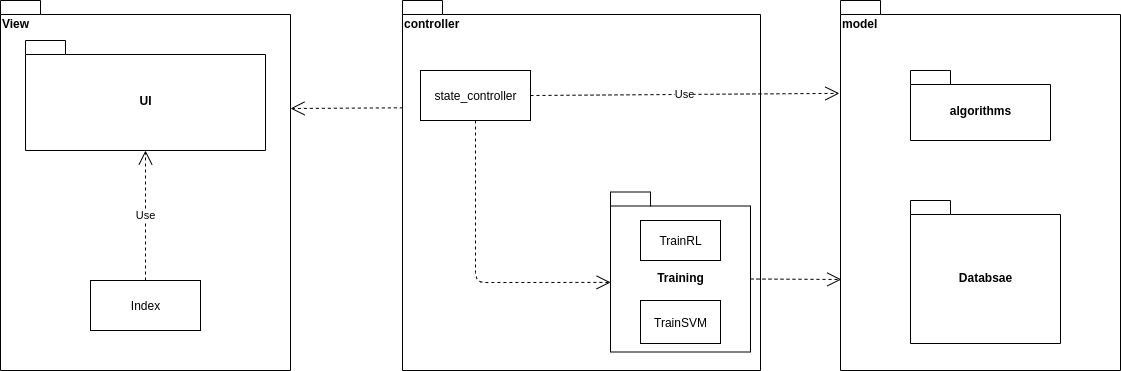
\includegraphics[scale=0.40]{../../Diagrams/Package_diagrams/plugin_design_pattern.png}
\caption{Diagramma dei package del Prediction Plug-in}
\end{figure}

\subsubsection{Diagrammi delle classi}
\textbf{Model}
\begin{figure}[H]
\centering
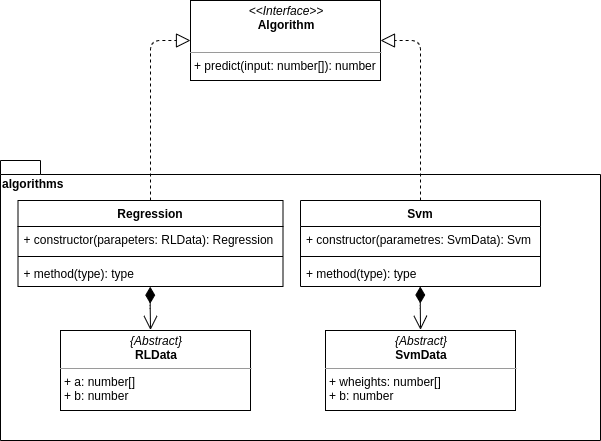
\includegraphics[scale=0.5]{../../Diagrams/Classes_diagrams/plugin_model.png}
\caption{Diagramma delle classi del Model del Prediction Plug-in}
\end{figure}

\textbf{View}
\begin{figure}[H]
\centering
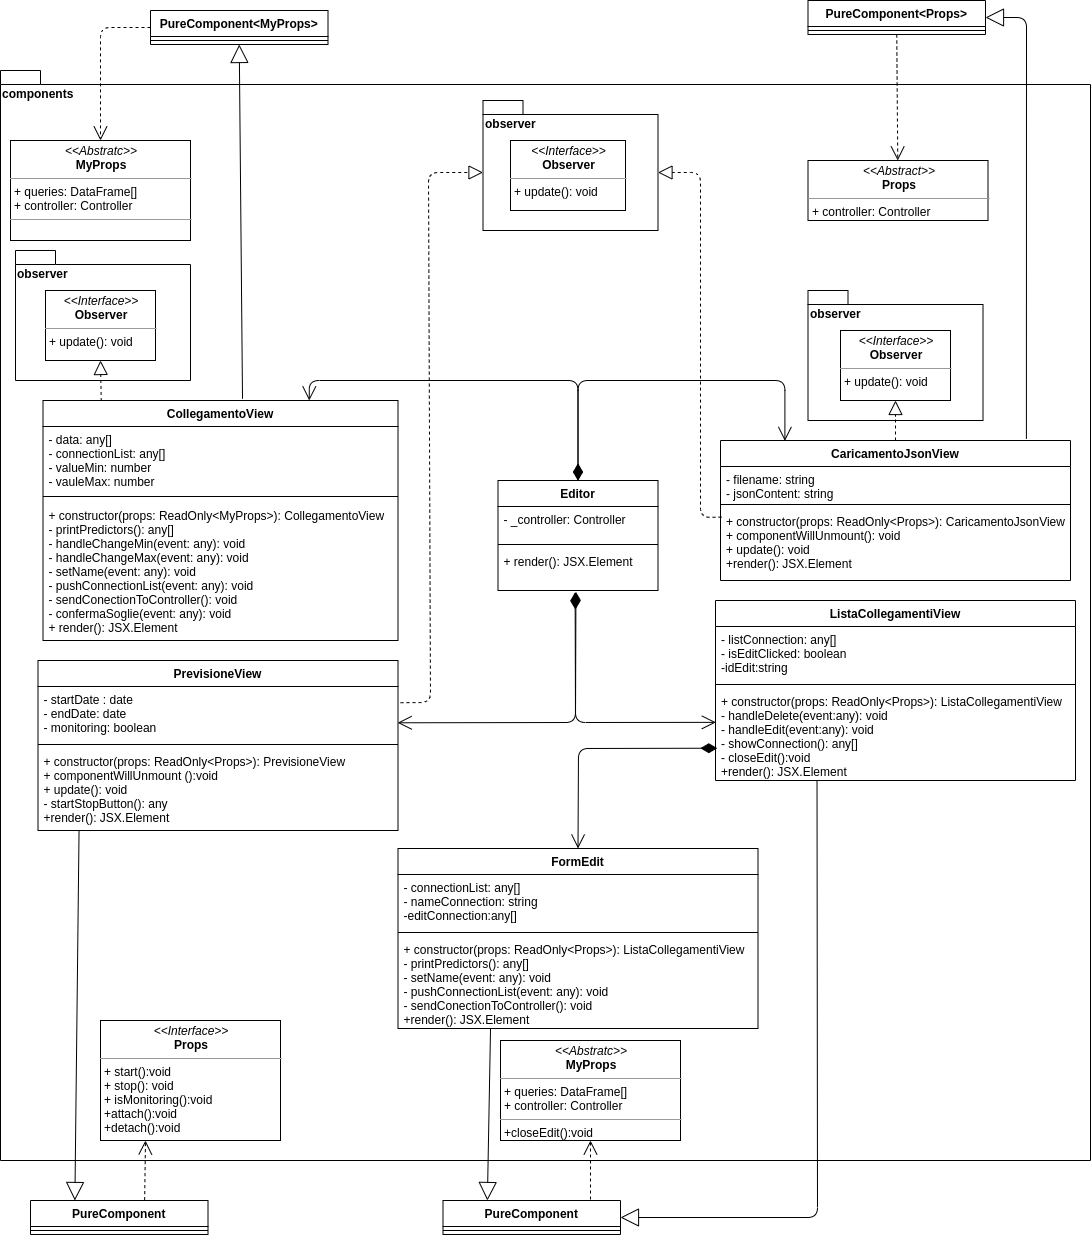
\includegraphics[scale=0.4]{../../Diagrams/Classes_diagrams/plugin_view.png}
\caption{Diagramma delle classi della View del Prediction Plug-in}
\end{figure}

\textbf{Controller}
\begin{figure}[H]
\centering
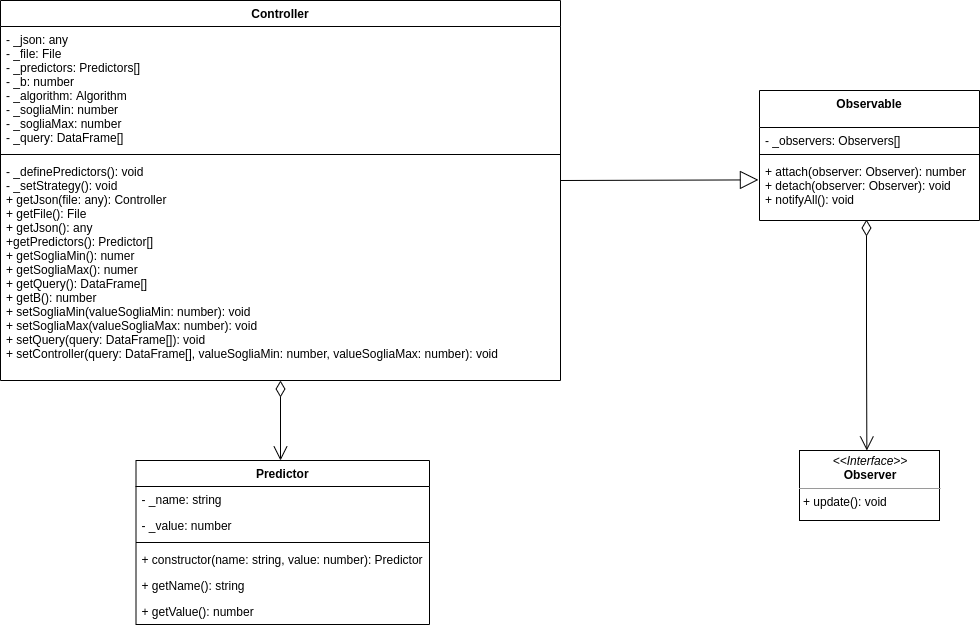
\includegraphics[scale=0.4]{../../Diagrams/Classes_diagrams/plugin_controller.png}
\caption{Diagramma delle classi del Controller del Prediction Plug-in}
\end{figure}

\subsubsection{Diagrammi di sequenza}

\subsubsection{Design pattern notevoli utilizzati}

